This chapter gives a theoretical overview of the issue of content profiling for digital preservation. It summarises the goals and requirements of the process. Then a detailed definition of the preservation planning process is given, followed by the relation of content profiling to digital preservation and how it fits in the bigger picture. The chapter defines the content profiling process and its necessary steps as well as gives insight into the importance and theory of representative sets. At the end, the topic of continuous profiling and its benefit to preservation systems and experts is discussed shortly.

\section {Goals}
\label{sec:goals}
Content Profiling makes use of the output of low-level technical processes and transforms it into input for the high-level decision making process of preservation planning.

Lower level technical processes such as characterisation play an important role not only to preservation planning but to DP in general. These processes have to deal with single objects (even though the scale can be very large). As output they provide information to quality assurance activities and workflows as well as preservation planning. The identity and meta data extracted out of every single digital object is the scaffold that enables many other processes and applications to do their work. Consequently, the tools that provide this data care the responsibility for any subsequent process that relies on this data and its validity.

Preservation planning is a higher level process that acts upon sets of objects. As such, preservation planning deals with large volumes of data, but is responsible that every single object complies to the requirements of a preservation expert after a preservation action is conducted. The usual size of real world-scenario collections does not allow the test and inspection of every single object before and after each evaluated preservation action. Thus, a bigger picture of the content at hand plays an immense role in the choosing of representative samples and implicitly on the decision made by a preservation expert.

In order to ensure that these two different important parts of Digital Preservation fit together and provide a valid and effective outcome, an adaptor is needed. It has to transform the fine granular output of one process into an aggregated higher level input to the other.

Identification and characterisation are technical processes that can be conducted in automated fashion. Preservation Planning, on the other hand, is a process which can be automated only to a certain extent and will always rely on a human decision. Nonetheless, the degree of automation can be highly improved as the current state of the art is. 

A huge problem lies in the fact, that meta data extracting tool often provide data, that is not necessarily valid. The sparsity of the data presents another difficult task when evaluating content during preservation analysis and makes it even more difficult to grasp the peculiarities of the content. The volumes of the content and even of the meta data are high enough to present scalability challenges and sometimes even to dub the processing infeasible.

All these issues outline the goals of the content profiling process, which are summarised as follows:

\begin{itemize}
\item Enable automatic and scalable aggregation of sparse meta data provided by identification and characterisation tools.
\item Create and expose a well-defined, machine readable footprint of the content at hand, for other actors to use. This has to summarise the following information.
 \begin{itemize}
  \item an identifier of the content or collection.
  \item the characteristics of the content, such as mime types, formats, size, but also any other that is of interest to preservation planning.
  \item a set of sample records.
  \item the scope of the profile (e.g. the object identifiers of the collection, within a repository interface) or some other means to distinguish the objects that conform to this profile.
 \end{itemize}
\item Enable planning experts to analyse the content. This includes:
 \begin{itemize}
  \item obtaining an overview of the content types and formats, of the collection, but is not restricted only to these.
  \item generating statistical reports about the size of the content.
  \item filtering the content into homogeneous sub sets, based on multiple characteristics.
 \end{itemize}
\item Export the raw (sparse) meta data in a common format that can be processed by other analysis software, which will enable preservation experts to conduct even more in-depth analysis.
\item Select representative subsets based on different approaches, that make sense in different planning use cases.
\item Browse the raw meta data of objects.
\end{itemize}

\section{Profiling}
\label{sec:content_profiling}
This section describes content profiling and discusses its prerequisites and requirements. Afterwards it proposes an approach of creating a profile in an automatic fashion. Subsequently the enhancement of preservation planning through automation support during analysis of content in real world DP scenarios and integration with other DP information systems is discussed.

\subsection{Prerequisites}
In order to generate a good and valid content profile some requirements have to be met. For one, the characterisation has to be provided, but also its data quality in terms of validity, normalisation, etc. has to be guaranteed.

\subsubsection{Characterisation Data}
Clearly, to profile a set of digital objects, the meta data of the set of objects are needed. There are arguments whether or not the characterisation process should be part of profiling. We support the opinion, that characterisation should be done before and its output serves as input to a profiler. There are two main reasons for this. One, in real world scenarios content is usually stored in special archives (digital repositories), which extract the meta data out of the digital objects upon ingest in these systems. Thus, it does not make sense to access the original objects again and run a potentially time-consuming process over them again. The second reason is that profiling is an analysis step and should not make use of one characterisation tool, but should try to be agnostic to the meta data format. After all meta data are just key-value pairs. It is much better to support different formats and transform them to an internal model instead of restricting the whole process to one format.

\subsubsection{Data \& Normalisation}
In order to achieve the goals outlined above, the meta data provided by the characterisation tools has to be normalised and should fit into a unified model no matter its origin.

Consider the following example. Two characterisation tools provide meta data for document formats and measure different characteristics for these documents but one - the number of embedded tables in the document. Only, the first tool reports this characteristic under the name \textit{'tableCount'} and the second \textit{'nrTables'}. Semantically both measures provide the same information. Thus it will be very valuable to a planner to know if both tools provided the same result or not. The coverage of this property within the characterised set will be potentially higher, since characterisation tools do not often manage to extract every property out of every digital object.

This example reveals two problems. Firstly, if the data is not normalised at all, the sparsity will be even higher and this will compromise the analysis and the gained knowledge about the collection. The second problem is the difficulty of normalisation itself. In the given example, it is fairly easy to assume that the semantics of the given property are the same. However, this is not true for all characteristics of all properties. Correct normalisation requires the domain knowledge of DP experts, the developers of the characterisation tool and potentially other experts. If it is done wrong, the whole result of a profile can be compromised.

Because of these problems, it is very important that characterisation tools provide valid and well-documented data. On the other hand, profiling tools should allow the normalisation of such data if the characteristics are well-defined and it is clear that the semantics of two or more properties are the same.

For this purpose, a simple but flexible domain model has to be created that allows properties, their measurements, provenance information and more to be stored at one place. The data structure has to enable efficient aggregation and querying of the data. Important aspects that have to be taken into consideration during design are the sparsity of the meta data, the different data types of the measurements. As discussed, the validity of measurements is often unreliable, so it is important to keep the provenance information of the measurements. If the profiler is ought to keep track of continuous data, then the time of measurement should also be taken into account. Another important issue is the identifier of each object, which has to be able to point to the original in the repository system.

%Another important aspect of the data is its validity. Obviously if the data that is provided is valid and of high quality, then the created profiles and the chosen representative sample objects will solely rely on the processes and algorithms involved. If these processes and algorithms are validated and on their terms of high quality, then the result will be a profile that enables unbiased experiments in preservation planning activities. As profiling depends on the meta data and the tools that are able to extract it, it is of great importance that quality assurance is conducted. Unfortunately, the state of the art does not provide many methods of checking the validity of a characterisation tool. %cite? qa in characterization?
% why is it important (iteration of before)

\subsection{The process}
Content profiling consists of three main parts; data harvesting, data aggregation and analysis. These are illustrated in Figure \ref{fig:cp_threesteps} and is discussed in the following.

\begin{figure}[bh]
\begin{center}
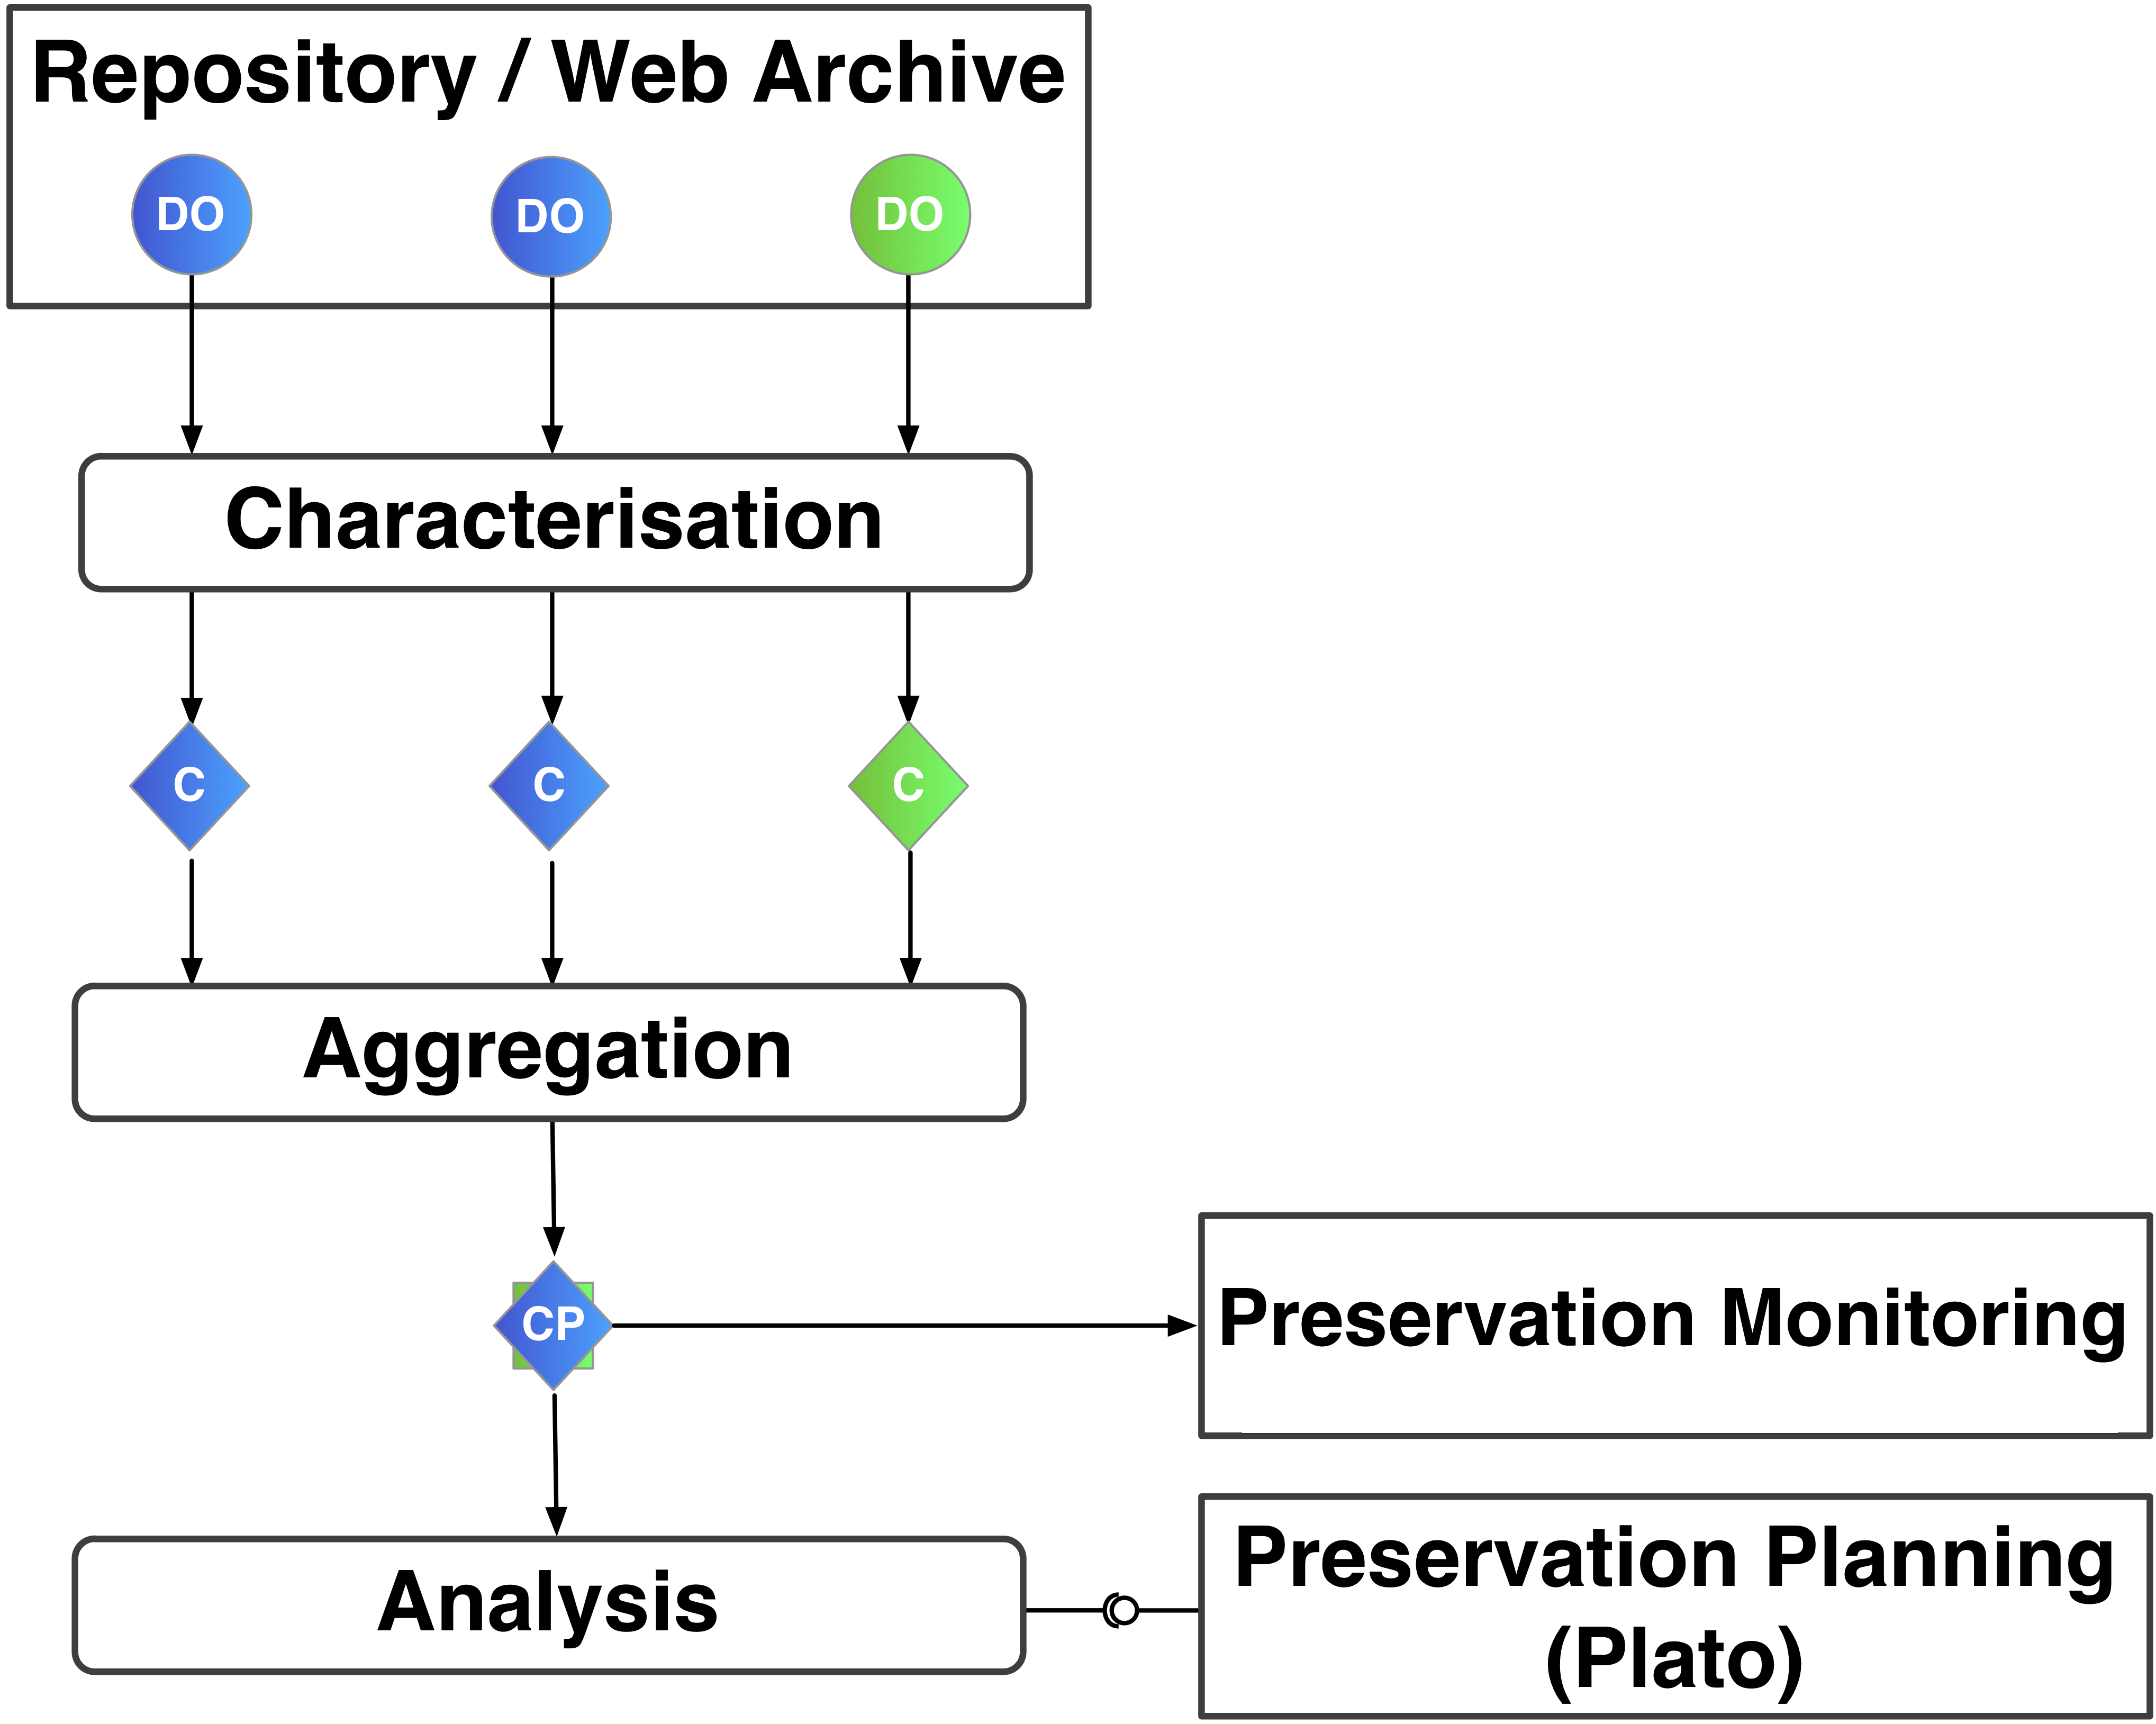
\includegraphics[width=3in]{figures/contentprofiling/contentprofiling.png}
\caption{The three steps of content profiling}
\label{fig:cp_threesteps}
\end{center}
\end{figure}

The first step is responsible for characterising, collecting and processing the digital objects (DO) in a DP system and adapting it to the internal model of the profile framework. This includes normalisation of the different properties and characteristics, removal of unnecessary data and more. Since DP scenarios usually make use of digital repositories, it should be possible to harvest the meta data directly from the repository. This can present a potential issue, due to the differences in the interfaces of repositories. Nonetheless, it has to be considered within the design of the system. Of course the approach could include characterisation as part of the process, which would result in a collection of meta data files. In such a case, the disadvantages discussed above, should be considered. After extracting and parsing the characterisation data out of the digital objects, special post-processing steps can be applied to each meta data object in order to refine the gathered data. For example, if the characterisation process does not provide normalised data, special actions can be undertaken to deal with this issue. Also, if there are conflicted values of the same property provided by different meta data sources, data cleanup actions and rules can be executed. These post-processing steps can have huge impact on the final result and thus should not be executed lightly, but only through special configuration steps, done by preservation experts, that understand the source of the meta data, the operations of the identification and characterisation tools and the implications of such alterations of the data. Thus, such functionality of the content profiler has to be done in a flexible fashion and has to allow special configuration that can alter and turn on and off such behaviour. Once the data fits the internal representation of the profiler, it can be stored in a data base per digital object level and thus allow further processing by the profiling process.

The next step of aggregation can be done either after the characterisation data (C) is parsed, normalised and stored or on demand if the underlying data store provides the necessary facilities. It is responsible to present the big picture of the data in a smaller footprint and structured form, so that other programs and tools can integrate with it. This content profile (CP) should provide enough flexibility to understand the data but also be aggregated as much as possible. Here different queries and aggregations can be executed, stored or cached in order to enable analysis or export of the data. An important issue that has to be considered is how the content profile data is going to be kept in sync during longer timeframes and after content changes. 

The last step is a higher level service on top of the framework, that has to be conducted mostly manually by the preservation expert. This means that it will rely on specific decisions and will need the input of a user. Nonetheless, it should be automated as much as possible and shall support the user in her decisions. This includes querying the data and gaining knowledge about the content by drilling it down based on different characteristics, but also the export of the whole raw data or a subset of it in a representation that allows further analysis but provides comprehensible overview.
Due to the nature of the data (a set of key-value pairs per object), a sparse matrix seems to be a good fit for this.

\subsection{Limitations \& Pitfalls}
There are a number of problems and potential pitfalls, that have to be considered when designing and implementing the proposed framework.

A very important issue is the removal of objects. It is, unusual that objects are removed from archives, but it is not impossible (e.g. after migration). Once an object (or a set of objects) is removed, the profile may become invalid and should be regenerated. If the source system (repository, file system, etc) does not provide information of which objects were deleted, the whole process should be repeated from the beginning. This could be time and resource consuming.

The same holds if new meta data is acquired and merged within the current profile. Here normalisation has to be kept intact and also any aggregation that might be influenced should be recalculated.

Clearly, the quality of a content profile is highly dependant on the quality of meta data, which makes it very important for preservation experts to know and understand the identification and characterisation tools they use.

If data normalisation is done via the framework and is not part of the meta data input, then very specific expertise will be required to do this task efficiently.

\subsection{Output}
% specification (representation, xml, rdf)
The profiler has to present the aggregated data in a form that is usable to planning experts, but also allow the export of the data into other formats for further processing. Furthermore, the preservation process will be enhanced, only if the data
can be obtained in a machine readable format, so that other tools can interact with it.

There are numerous ways of representing such a profile. However, from the observations of the previous chapter there are number of goals that it has to fulfil. It has to follow a well-defined schema; the profile has to be in a structured, machine readable form, as it will act as input to other information systems in the DP landscape.

Clearly, it has to aggregate the raw data, so that it has a small enough footprint, but still provide enough insight into the content at hand. The profile should be able to separate the content based on different characteristics. Here it is important that a user or a user application is able to go one step back and examine the filtering criteria. Finally, the profile should include a small set of representative objects, with their full characteristics and a way to identify all objects in a set or collection that fit into the specified filter. The latter could be done, either via some kind of query or just by a list of objects outlines the identifiers of all selected objects.

Having such a content profile is the foundation for integration with other DP software systems, such as preservation watch and monitoring systems, simulation environments and planning components. For this integration some higher level features based on the exported profile and representative sets can be done.

%Appendix A shows a proposal of the first format schema.

\section{Continuos Profiling}
A content profiler tool can provide benefit to numerous systems and users in a Digital Preservation environment. On the one hand, it can act as direct input to Preservation Planning and can spare a planning expert a lot of time defining and outlining a plan. On the other hand, it supplies the needed foundation to do continuous profiling. Continuous profiling refers to two higher level applications of content profiling when integrating with other systems. The one is profiling data based on its creation or harvesting date. The other one is the continuous monitoring of a profile of a collection and all its changes through time. Here we give some overview of both ideas and summarise how these can be achieved and what benefits they will provide to planning experts.

\subsection{Monitoring}
As discussed in the previous chapter monitoring is an external phase of the preservation planning environment that provides feedback and can trigger reevaluation of a plan. If a content profile generated from the content of a repository is observed continuously by such a monitoring system, then certain triggers can be raised when conditions are met or constraints violated.
For example, an organisation that may have a policy that defines which objects have to be preserved and one that defines how many objects of a certain type can exist without a valid plan associated to them. Now consider that each day a great deal of new objects is ingested into the repository of that particular organisation. By the end of a certain time period a content profile is regenerated and a monitoring system obtains and reevaluates this result against the organisational policies. It will be fairly easy to detect a potential mismatch and to notify the involved stakeholders and actors in order to resolve it, provided all of these pieces of the puzzle fit together.

Another great deal of the combination of such a content profile and monitoring system can be a global content profile. If enough organisations, such as Web Archives, Libraries, etc. are willing to share the profiles (or parts of them) they have with such a central monitor, the result will most probably be a representative overview of the global state of the world \cite{becker-ipres2012}. Valuable information, such as the number of formats used within a certain domain, the preferred type of files within a user community, the emergence of new file formats, the decline of old file formats and much more can be detected. Provided that enough content-holding institutions are ready to sacrifice a bit of their privacy, the mutual benefit could be something much more valuable.

The integration between a content profiling tool and such a monitoring system presents some technical issues and questions that have to be answered, as content holding institutions make use of different repository and systems. Nonetheless, if there is a profiling tool running within such a system or near the data and conforms to a standardised machine-readable output, then such an integration is feasible. A design proposition of such a novel preservation watch system is discussed in \cite{duretec:2012:watch, FariaPDBFR12}.


%TODO
%describe minitoring
% how does it work in terms of content profiling
% need of an exposed service
% cite papers at the according places and may be not up there

\subsection{Simulation \& Trend Analysis}
Content profiling can be integrated with simulation software that tries to analyse the trends of different characteristics of the content over time such as future development of format profiles, detection of format obsolescence and emerging formats, size fluctuations, or any other preservation related characteristic.

Weihs et.al demonstrate a simulation prototype \cite{TUW-206758} that can simulate the evolution of a repository over time. The input used for the simulations are different models and configurations of the content, as well as the potential result of preservation actions over this content. An integration between such a tool and a real world content profile is an approach to examine and validate how simulation influences digital preservation decisions, but also provide new requirements and goals for content profiling  as well.

Other interesting aspects to simulate include the format profile of a repository over time. There are different theories regarding the lifetime of formats and a debate pro and contra for following a direct migration strategy or whether or not this should be left to the so called network effects of data sharing, which should prevent the damages of obsolescence \cite{Rosenthal:1January2010:0737-8831:195}. Jackson gives a good summary of this debate and asks the question: ''Where is the evidence?'' In order to find out, experiments of format usage over large digital corpora of the British Web Archive are conducted. The results are presented in \cite{journals/corr/abs-1210-1714} and suggest that there are indeed formats that live longer than five years, however there were a number of formats fading from use and these should be studied closely. Apart from being very interesting, these (unstructured) profiles could act as input to simulation environments, where based on the past trends new hypothesis for the future development are tested and used for planning. Another interesting aspect is the differentiation between use of formats in production and in access. There are certain formats, where production declines rapidly and still there is a great deal of rendering software that enables the access of the existing content. The question remains, whether a format is obsolete when evidence for its production stops or when it cannot be accessed and rendered correctly or a combination of both.

One example of such trend results is presented in Figure \ref{fig:trends_html}. There the different html versions of about 1.5 million webarchive digital objects from the the danish web archive are presented through the years. The data for this graph was processed with the help of the backend of a content profile tool following the suggested approach in this chapter. It was produced for another thesis conducted at the time of writing at the University of Technology in Vienna that researches different statistical trend analysis approaches for preservation. Thus, we believe that such content profiling output data can be of very high value to DP activities if it can be structured and processed by other software.

% Simulation environments
% cite or refer to Stefan Schindlers thesis and give him credit
% may be say that this was possible with the backend of the tool presented in the next chapter.

\begin{figure}[t]
\begin{center}
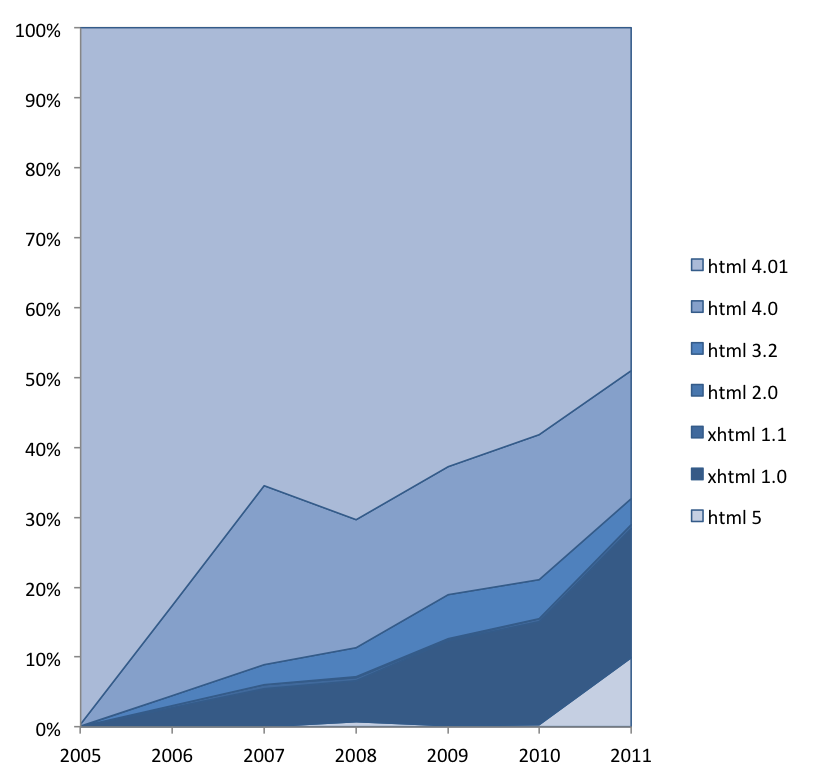
\includegraphics[width=3.6in]{figures/contentprofiling/trends_html.png}
\caption{Usage trends in html versions over time in a danish web archive}
\label{fig:trends_html}
\end{center}
\end{figure}

\section{Representative Sets}
\label{sec:representative_sets}
% what is the problem,
% how do we create them/find them
As discussed in Section \ref{lbl:preservationplanning} finding a small set of representative sample objects is one of the most important steps during the first step of the planning process as it forms the foundation for the chosen course of action.

The goal is to choose a small set of objects out of a much larger set.
This small set should ideally capture the essence of the large set, which means covering as much of the different measurements of a set of characteristics \cite{Becker:2011:PDT:1998076.1998089}.

There are a couple of questions that a preservation planner has to answer when selecting this set.
Firstly, how many samples is enough?
And secondly, what characteristics are important for the coverage?

Unfortunately, both of these questions do not have specific answers and are highly dependent on the given preservation use case.
Nonetheless, these questions outline some requirements for the planner to consider during selection and planning.
The sample set has to have as few as possible entries due to the resource consumption of the experiments, but as many as needed to guarantee the validity of the experiments.
As far as the characteristics are concerned, the planner has to select such characteristics that are important for the use case, that are measurable and could cover as much as possible in the set.
Consider a collection that is homogeneous in terms of the format.
Choosing your samples based on the format would not make much sense, as the chosen samples would still be random due to the format homogeneity.

Choosing such samples is somehow related to the more known problem of clustering.
Clustering tries to organise a given set of patterns based on similarity, usually by representing them in vectors or points in multidimensional spaces and their distances \cite{Jain:1999:DCR:331499.331504}.
The problem is that we do not only search for similar objects based on different characteristics, but we want to select enough objects of every distinct cluster, so that we have the confidence that enough objects were selected to cover all peculiarities and differences between them, that could be the cause of a failure.
To some extent the first step of filtering through the content and finding a homogeneous set is the clustering, which results   in one cluster of the whole content. The representative sample set is a much smaller subset in this cluster that has to cover as much as possible of the differences between the objects inside of the homogeneous set. Clearly, if the first step is omitted, finding a representative set, should still work. However, it will be more complex to achieve a good coverage as the differences will be much more as well as the data sparsity will be larger. 